\documentclass[a4paper,12pt]{article} 

%%% Работа с русским языком
\usepackage{cmap}					% поиск в PDF
\usepackage{mathtext} 				% русские буквы в фомулах
\usepackage[T2A]{fontenc}			% кодировка
\usepackage[utf8]{inputenc}			% кодировка исходного текста
\usepackage[english,russian]{babel}	% локализация и переносы

%%% Дополнительная работа с математикой
\usepackage{amsmath,amsfonts,amssymb,amsthm,mathtools, gensymb} % AMS
\usepackage{icomma} % "Умная" запятая: $0,2$    ф--- число, $0, 2$ --- перечисление

%%Таблица
\usepackage[table,xcdraw]{xcolor}
\usepackage{caption}
\usepackage{floatrow}
\floatsetup[table]{capposition=top}
\floatsetup[wrapfigure]{capposition=bottom}

%Отступы и поля 
\textwidth=18cm
\oddsidemargin=-1cm
\topmargin=-2cm
\textheight=25cm


%% Номера формул
\mathtoolsset{showonlyrefs=true} % Показывать номера только у тех формул, на которые есть \eqref{} в тексте.

%% Шрифты
\usepackage{euscript}	 % Шрифт Евклид
\usepackage{mathrsfs} % Красивый матшрифт

%% Свои команды
\DeclareMathOperator{\sgn}{\mathop{sgn}}

%% Перенос знаков в формулах (по Львовскому)
\newcommand*{\hm}[1]{#1\nobreak\discretionary{}
{\hbox{$\mathsurround=0pt #1$}}{}}

%% Стиль страницы
\usepackage{fancyhdr}

%% Для рисунков
\usepackage{graphicx}
\usepackage[export]{adjustbox}
\usepackage{float}
\usepackage{ragged2e}
\usepackage{wrapfig}

\pagestyle{fancy}
\begin{document}
\begin{titlepage}
\begin{center}
%\vspace*{1cm}
\large{\small ФЕДЕРАЛЬНОЕ ГОСУДАРСТВЕННОЕ АВТОНОМНОЕ ОБРАЗОВАТЕЛЬНОЕ\\ УЧРЕЖДЕНИЕ ВЫСШЕГО ОБРАЗОВАНИЯ \\ МОСКОВСКИЙ ФИЗИКО-ТЕХНИЧЕСКИЙ ИНСТИТУТ\\ (НАЦИОНАЛЬНЫЙ ИССЛЕДОВАТЕЛЬСКИЙ УНИВЕРСИТЕТ)\\ ФАКУЛЬТЕТ АЭРОКОСМИЧЕСКИХ ТЕХНОЛОГИЙ}
\vfill
\line(1,0){490}\\[1mm]
\huge{Лабораторная работа 3.3.5}\\
\huge\textbf{Эффект Холла в металлах}\\
\line(1,0){490}\\[1mm]
\vfill
\begin{flushright}
\normalsize{Рогозин Владимир}\\
\normalsize{\textbf{Группа Б03-106}}\\
\end{flushright}
\end{center}
\end{titlepage}
\fancyhead[L] {Работа 3.3.5}


\textbf{Цель работы}: 
измерение подвижности и концентрации носителей заряда в металлах.

\textbf{Оборудование}:
электромагнит с источником питания, источник постоянного тока, микровольтметр, амперметры, милливеберметр или цифровой магнитометр, образцы из меди, серебра и цинка.

\textbf{Теоретические сведения}: 

В работе изучаются особенности проводимости металлов в геометрии мостика Холла. Ток пропускается по плоской прямоугольной металлической пластинке, помещённой в перпендикулярное пластинке магнитное поле. Измеряется разность потенциалов между краями пластинки в поперечном к току направлении. По измерениям определяется константа Холла, тип проводимости и вычисляется концентрация основных носителей заряда.

Во внешнем магнитном поле $\mathbf{B}$ на заряды действует сила Лоренца:
\[\mathbf{F} = q\mathbf{E} + q \mathbf{u} \times \mathbf{B}.\]
Эта сила вызывает движение носителей, направление которого в общем
случае не совпадает с $\mathbf{E}$. Траектории частиц будут либо искривляться, либо, если геометрия проводника этого не позволяет, возникнет дополнительное электрическое поле, компенсирующее магнитную составляющую силы Лоренца. Возникновение поперечного току электрического поля в образце, помещённом во внешнее магнитное поле, называют \textit{эффектом Холла}.

Связь между электрическим полем $\mathbf{E}$ и плотностью тока $\mathbf{j}$ в условиях эффекта Холла уже не может быть описана скалярным коэффициентом
проводимости $\sigma$. Тем не менее закон Ома можно по-прежнему записать в форме
\[\mathbf{j} = \hat{\sigma} \mathbf{E},\]
если под $\hat{\sigma}$ понимать тензор проводимости. В заданном базисе он
представляется матрицей \\ 3 $\times$ 3:
\begin{equation}
    \mathbf{j} = \hat{\sigma} \mathbf{E} = 
        \begin{pmatrix}
                \sigma_{xx} & \sigma_{xx} & \sigma_{xz} \\
                \sigma_{yx} & \sigma_{yy} & \sigma_{yz} \\
                \sigma_{zx} & \sigma_{zy} & \sigma_{zz} \\
        \end{pmatrix} \mathbf{E}.
\end{equation}
или
\[j_i = \sum_k \sigma_{ik} E_k, \quad \text{где } i, k = \{x, y, z\}.\]
Тензорная связь между полем и током имеет место в общем случае, когда проводящая среда не является изотропной. В условиях эффекта Холла тензор проводимости становится недиагональным.

Пусть система содержит носители только одного типа (например,
электроны, как в большинстве металлов). Рассмотрим сначала простейший случай плоской геометрии: пусть ток течёт вдоль оси $x$, а магнитное поле направлено вдоль оси $z$. Магнитное поле действует на движущиеся заряды с силой $F_y = -q u_x B_z$.  Ток сможет течь строго вдоль оси $x$, если заряды в среде перераспределятся таким образом, чтобы полностью скомпенсировать магнитную силу, создав в направлении $y$ электрическое поле
\[E_y = u_x B_z = \frac{j_x}{nq} B_z\]
называемое \textit{холловским} (здесь $n$ -- концентрация носителей). По оси
$x$ носители будут двигаться так, как если бы магнитного поля не было:
$j_x = \sigma_0 E_x$ ($j_y = j_z = 0$), где $\sigma_0 = q n \mu$ -- удельная проводимость среды в отсутствие $\mathbf{B}$.
\begin{figure}[H]\label{fig: electron in B and E}
    \centering
    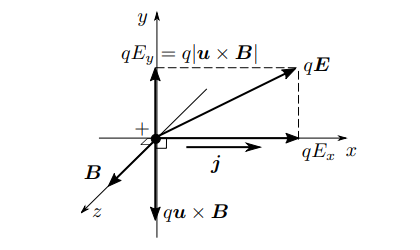
\includegraphics[scale = 0.95]{Частица в полях.png}
    \caption{Силы, действующие на положительный носитель заряда в проводящей среде при наличии магнитного поля}
\end{figure}

Выразим общую связь между $\mathbf{j}$ и $\mathbf{E}$ для случая носителей одного типа. Магнитное поле по-прежнему направим вдоль оси $z$, а о направлении $\mathbf{j}$ и $\mathbf{E}$ никаких предположений делать не будем. При движении носителей с постоянной средней скоростью сила Лоренца будет уравновешена трением со стороны среды:
\[q(\mathbf{E} + \mathbf{u} \times \mathbf{B}) - \frac{q \mathbf{u}}{\mu} = 0\]
С учётом введённых выше обозначений этот баланс сил можно переписать как
\[\mathbf{E} = \frac{\mathbf{j}}{\sigma_0} - \frac{1}{nq} \mathbf{j} \times \mathbf{B}.\]
Полученное соотношение можно назвать обобщённым законом Ома при наличии внешнего магнитного поля. Второе слагаемое в правой части как раз отвечает эффекту Холла -- возникновению поперечного направлению тока электрического поля.

Записывая равенство по компонентам
\[E_x = \frac{j_x}{\sigma_0} - \frac{j_y B}{nq}, \quad E_y = \frac{j_y}{\sigma_0} + \frac{j_x B}{nq}, \quad E_z = \frac{j_z}{\sigma_0}\]
получим, вводя \textit{тензор удельного сопротивления} $\hat{\rho}$
\begin{equation}
    \mathbf{E} = \hat{\rho} \mathbf{j} = \begin{pmatrix}
                                        1 & -\mu B & 0 \\
                                        \mu B & 1 & 0 \\
                                        0 & 0 & 1\\
    \end{pmatrix} \frac{\mathbf{j}}{\sigma_0}
\end{equation}
Обращением матрицы получим тензор проводимости в условиях эффекта Холла:
\begin{equation}
    \hat{\sigma} = \hat{\rho}^{-1} = \frac{\sigma_0}{1 + (\mu B)^2} \begin{pmatrix}
        1 & \mu B & 0\\
        -\mu B & 1 & 0\\
        0 & 0 & 1 + (\mu B)^2\\
    \end{pmatrix}
\end{equation}
Безразмерному параметру $\mu B$ можно приписать простой физический смысл — это отношение эффективной длины пробега частиц $l = \mu m u / q$ к ларморовскому радиусу кривизны их траектории $r_B = m u / q B$. Эту величину иногда называют \textit{параметром замагниченности}.

\textbf{Мостик Холла.}
\begin{figure}[H]\label{fig: mostik Holla}
    \centering
    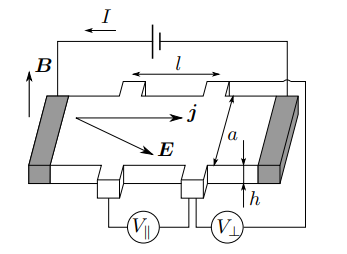
\includegraphics[scale = 0.95]{Мостик Холла.png}
    \caption{Схема для исследования влияния магнитного поля на проводящие свойства: мостик Холла}
\end{figure}
В данной схеме ток вынуждают течь по оси $x$ вдоль плоской пластинки  (ширина пластинки $a$, толщина $h$, длина $l$). Сила Лоренца, действующая со стороны перпендикулярного пластинке магнитного поля, «прибивает» носители заряда к краям образца, что создаёт холловское электрическое поле, компенсирующее эту силу. Поперечное напряжение между краями пластинки (холловское напряжение) равно $U_{\perp} = E_y a$, где
\[E_y = \rho_{yx} \cdot j_x = \frac{j_x B}{nq}.\]
Плотность тока, текущего через образец, равна $j_x = I / ah$ где $I$ -- полный ток, $ah$ -- поперечное сечение. Таким образом, для холловского напряжения имеем
\[U_{\perp} = \frac{B}{nqh} \cdot I = R_{H} \cdot \frac{B}{h} \cdot I\]
где константу
\[R_{H} = \frac{1}{nq}\]
называют \textit{постоянной Холла}. Знак постоянной Холла определяется знаком заряда носителей.

Продольная напряжённость электрического поля равна
\[E_x = \rho_{xx} \cdot j_x = j_x / \sigma_0\]
и падение напряжения $U_{\|} = E_x l$ вдоль пластинки определяется омическим сопротивлением образца $R_0 = l / (\sigma_0 a h)$:
\[U_{\|} = I R_0\]
Интересно отметить, что несмотря на то, что тензор проводимости явно зависит от $B$, продольное сопротивление образца в данной геометрии от магнитного поля не зависит.

\textbf{Экспериментальная установка}:
\begin{figure}[H]\label{fig: ustanovka}
    \centering
    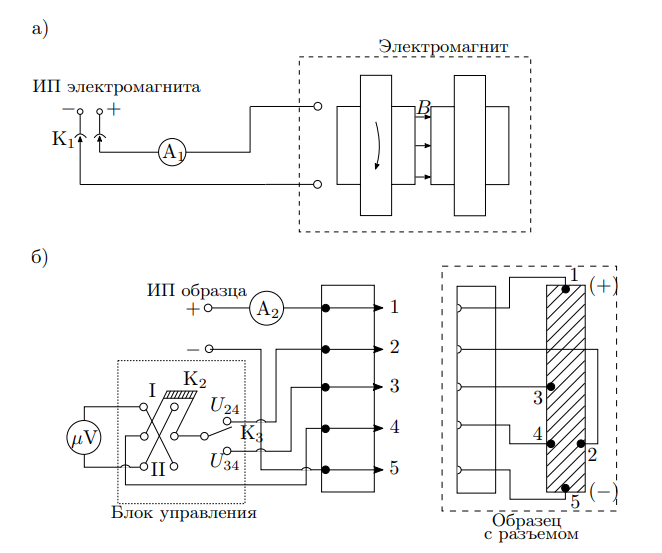
\includegraphics[width = 0.8\textwidth]{Установка.png}
    \caption{Схема установки для исследования эффекта Холла в металлах}
\end{figure}
Электрическая схема установки для измерения ЭДС Холла представлена на рис. 3. В зазоре электромагнита (рис. 3а) создаётся постоянное магнитное поле, величину которого можно менять с помощью источника питания электромагнита. Разъём $K_1$ позволяет менять направление тока в обмотках электромагнита. Ток питания электромагнита измеряется амперметром $A_1$

Градуировка электромагнита проводится при помощи  миллитесламетра на основе датчика Холла.

Металлические образцы в форме тонких пластинок, смонтированные в специальных держателях, подключаются к блоку питания через разъём (рис. 3б). Ток через образец регулируется ручками источника и измеряется амперметром $A_2$.

Для измерений ЭДС Холла используется микровольтметр, в котором
высокая чувствительность по напряжению сочетается с малой величиной тока, потребляемого измерительной схемой.

В образце с током, помещённом в зазор электромагнита, между контактами 2 и 4 возникает холловская разность потенциалов $U_{\perp}$, которая
измеряется с помощью микровольтметра, если переключатель $К_3$ подключён к точке 2 образца. При подключении $К_3$ к точке 3 микровольтметр измеряет омическое падение напряжения $U_{34}$, вызванное током через образец. При нейтральном положении ключа входная цепь микровольтметра разомкнута.

Ключ $К_2$ позволяет менять полярность напряжения, поступающего на вход микровольтметра.

Контакты 2 и 4 вследствие неточности подпайки могут лежать не на
одной эквипотенциали. Тогда напряжение между ними связано не только с эффектом Холла, но и с омическим падением напряжения вдоль пластинки. Исключить этот эффект можно если при каждом значении тока через образец измерять напряжение между точками 2 и 4 в отсутствие магнитного поля. При фиксированном токе через образец это дополнительное к ЭДС Холла напряжение $U_0$ остаётся неизменным. От него следует (с учётом знака) отсчитывать величину ЭДС Холла: 
\[U_{\perp} = U_{24} - U_0\]

При таком способе измерения нет необходимости проводить повторные измерения с противоположным направлением магнитного поля.

По знаку $U_{\perp}$ можно определить характер проводимости -- электронный или дырочный. Для этого необходимо знать направление тока в образце и направление магнитного поля.

Измерив ток $I$ в образце и напряжение $U_{34}$ между контактами 3 и 4
в отсутствие магнитного поля, можно, зная параметры образца, рассчитать удельное сопротивление $\rho_0$ и проводимость $\sigma_0$ материала образца по формуле
\[\rho_0 = \frac{U_{34} a h }{I l},\]
где $l$ -- расстояние между контактами 3 и 4, $a$ -- ширина образца, $h$ --
его толщина.


\textbf{Обработка данных}:  

Сначала определим максимальный ток через образец при напряжении $V = 0,8$ В, $I_{maxS} = 0,92$ А. Затем определим максимальный ток через катушку электромагнита при максимальном напряжении $U_{max} = 106,3$ В, $I_{maxM} = 1,35$ А.

Теперь проградуируем электромагнит, для этого, с помощью миллитесламетра, снимем зависимость магнитной индукции от силы тока в катушке увеличивая ток до максимального значения $I_{maxM}$. Результаты измерений приведены в таблице ниже. Абсолютная погрешность измерения силы тока в катушке равна 0,5\% + 2 ед. младшего разряда, абсолютная погрешность измерения индукции магнитного поля равна 5\% + 10 ед. младшего разряда.

\begin{table}[H]\label{tab: B(I)}
    \centering
    \begin{tabular}{|
        >{\columncolor[HTML]{FFFFFF}}c |
        >{\columncolor[HTML]{FFFFFF}}c |
        >{\columncolor[HTML]{FFFFFF}}c |
        >{\columncolor[HTML]{FFFFFF}}c |
        >{\columncolor[HTML]{FFFFFF}}c |
        >{\columncolor[HTML]{FFFFFF}}c |
        >{\columncolor[HTML]{FFFFFF}}c |
        >{\columncolor[HTML]{FFFFFF}}c |
        >{\columncolor[HTML]{FFFFFF}}c |}
        \hline
        {\color[HTML]{000000} $I$, А} &
          {\color[HTML]{000000} 0,16} &
          {\color[HTML]{000000} 0,32} &
          {\color[HTML]{000000} 0,48} &
          {\color[HTML]{000000} 0,64} &
          {\color[HTML]{000000} 0,80} &
          {\color[HTML]{000000} 0,96} &
          {\color[HTML]{000000} 1,12} &
          {\color[HTML]{000000} 1,28} \\ \hline
        {\color[HTML]{000000} $B$, мТл} &
          {\color[HTML]{000000} 147,7} &
          {\color[HTML]{000000} 309,5} &
          {\color[HTML]{000000} 458,0} &
          {\color[HTML]{000000} 606,6} &
          {\color[HTML]{000000} 758,6} &
          {\color[HTML]{000000} 930,4} &
          {\color[HTML]{000000} 1056,1} &
          {\color[HTML]{000000} 1132,9} \\ \hline
    \end{tabular}
    \caption{Зависимость магнитной индукции от силы тока}
\end{table}

По данным из таблицы построим график зависимости $B(I)$, определим коэффициент угла наклона.
\[k = (931,29 \pm 11,51) \text{ }мТл / А ,\quad \varepsilon_k = 1,24 \%\]

 Теперь приступим к измерению ЭДС Холла для образца из меди. Параметры образца:
 $L_{3,4} = 10$ мм, $h = 0,05$ мм, $l = 9$ мм. При одном значении тока в образце, изменяя ток в электромагните, будем менять величину магнитного поля и снимать зависимость ЭДС Холла от магнитной индукции, затем тоже самое проделаем для других значений тока в образце. Предел измерений микровольтметра -- 3 мкВ, цена деления -- 0,04 мкВ, погрешность измерений -- половина цены деления (0,02 мкВ). По данным из таблицы ниже для каждого из значений тока в образце построим графики зависимости ЭДС Холла $U_{\perp}$ от величины магнитного поля $B$. Каждую зависимость аппроксимируем прямой $y = kx$, для каждой прямой найдём угол её наклона. Результаты представлены в таблице ниже. 

 \begin{table}[H]\label{tab: UI Cu}
    \centering
    \begin{tabular}{|c|ccccccccc|}
        \hline
        \rowcolor[HTML]{FFFFFF} 
        {\color[HTML]{000000} $I_{обр}$, А} &
          \multicolumn{1}{c|}{\cellcolor[HTML]{FFFFFF}{\color[HTML]{000000} 0,2}} &
          \multicolumn{1}{c|}{\cellcolor[HTML]{FFFFFF}{\color[HTML]{000000} 0,3}} &
          \multicolumn{1}{c|}{\cellcolor[HTML]{FFFFFF}{\color[HTML]{000000} 0,4}} &
          \multicolumn{1}{c|}{\cellcolor[HTML]{FFFFFF}{\color[HTML]{000000} 0,5}} &
          \multicolumn{1}{c|}{\cellcolor[HTML]{FFFFFF}{\color[HTML]{000000} 0,6}} &
          \multicolumn{1}{c|}{\cellcolor[HTML]{FFFFFF}{\color[HTML]{000000} 0,7}} &
          \multicolumn{1}{c|}{\cellcolor[HTML]{FFFFFF}{\color[HTML]{000000} 0,8}} &
          \multicolumn{1}{c|}{\cellcolor[HTML]{FFFFFF}{\color[HTML]{000000} 0,9}} &
          {\color[HTML]{000000} 0,9} \\ \hline
        \rowcolor[HTML]{FFFFFF} 
        {\color[HTML]{000000} $U_0$,  дел.} &
          \multicolumn{1}{c|}{\cellcolor[HTML]{FFFFFF}{\color[HTML]{000000} 2,5}} &
          \multicolumn{1}{c|}{\cellcolor[HTML]{FFFFFF}{\color[HTML]{000000} 6,0}} &
          \multicolumn{1}{c|}{\cellcolor[HTML]{FFFFFF}{\color[HTML]{000000} 6,0}} &
          \multicolumn{1}{c|}{\cellcolor[HTML]{FFFFFF}{\color[HTML]{000000} 5,5}} &
          \multicolumn{1}{c|}{\cellcolor[HTML]{FFFFFF}{\color[HTML]{000000} 5,5}} &
          \multicolumn{1}{c|}{\cellcolor[HTML]{FFFFFF}{\color[HTML]{000000} 6,0}} &
          \multicolumn{1}{c|}{\cellcolor[HTML]{FFFFFF}{\color[HTML]{000000} 6,0}} &
          \multicolumn{1}{c|}{\cellcolor[HTML]{FFFFFF}{\color[HTML]{000000} 6,0}} &
          {\color[HTML]{000000} 6,0} \\ \hline
        \rowcolor[HTML]{FFFFFF} 
        {\color[HTML]{000000} $I_{кат}$, A} &
          \multicolumn{9}{c|}{\cellcolor[HTML]{FFFFFF}{\color[HTML]{000000} $U$, дел.}} \\ \hline
        \rowcolor[HTML]{FFFFFF} 
        {\color[HTML]{000000} 0,15} &
          \multicolumn{1}{c|}{\cellcolor[HTML]{FFFFFF}{\color[HTML]{000000} 7,0}} &
          \multicolumn{1}{c|}{\cellcolor[HTML]{FFFFFF}{\color[HTML]{000000} 8,0}} &
          \multicolumn{1}{c|}{\cellcolor[HTML]{FFFFFF}{\color[HTML]{000000} 8,0}} &
          \multicolumn{1}{c|}{\cellcolor[HTML]{FFFFFF}{\color[HTML]{000000} 8,0}} &
          \multicolumn{1}{c|}{\cellcolor[HTML]{FFFFFF}{\color[HTML]{000000} 9,0}} &
          \multicolumn{1}{c|}{\cellcolor[HTML]{FFFFFF}{\color[HTML]{000000} 10,0}} &
          \multicolumn{1}{c|}{\cellcolor[HTML]{FFFFFF}{\color[HTML]{000000} 11,0}} &
          \multicolumn{1}{c|}{\cellcolor[HTML]{FFFFFF}{\color[HTML]{000000} 12,0}} &
          {\color[HTML]{000000} 11,0} \\ \hline
        \rowcolor[HTML]{FFFFFF} 
        {\color[HTML]{000000} 0,30} &
          \multicolumn{1}{c|}{\cellcolor[HTML]{FFFFFF}{\color[HTML]{000000} 8,0}} &
          \multicolumn{1}{c|}{\cellcolor[HTML]{FFFFFF}{\color[HTML]{000000} 9,5}} &
          \multicolumn{1}{c|}{\cellcolor[HTML]{FFFFFF}{\color[HTML]{000000} 10,5}} &
          \multicolumn{1}{c|}{\cellcolor[HTML]{FFFFFF}{\color[HTML]{000000} 11,5}} &
          \multicolumn{1}{c|}{\cellcolor[HTML]{FFFFFF}{\color[HTML]{000000} 13,0}} &
          \multicolumn{1}{c|}{\cellcolor[HTML]{FFFFFF}{\color[HTML]{000000} 15,0}} &
          \multicolumn{1}{c|}{\cellcolor[HTML]{FFFFFF}{\color[HTML]{000000} 16,5}} &
          \multicolumn{1}{c|}{\cellcolor[HTML]{FFFFFF}{\color[HTML]{000000} 18,5}} &
          {\color[HTML]{000000} 17,5} \\ \hline
        \rowcolor[HTML]{FFFFFF} 
        {\color[HTML]{000000} 0,45} &
          \multicolumn{1}{c|}{\cellcolor[HTML]{FFFFFF}{\color[HTML]{000000} 9,0}} &
          \multicolumn{1}{c|}{\cellcolor[HTML]{FFFFFF}{\color[HTML]{000000} 11,5}} &
          \multicolumn{1}{c|}{\cellcolor[HTML]{FFFFFF}{\color[HTML]{000000} 12,5}} &
          \multicolumn{1}{c|}{\cellcolor[HTML]{FFFFFF}{\color[HTML]{000000} 15,0}} &
          \multicolumn{1}{c|}{\cellcolor[HTML]{FFFFFF}{\color[HTML]{000000} 17,0}} &
          \multicolumn{1}{c|}{\cellcolor[HTML]{FFFFFF}{\color[HTML]{000000} 19,0}} &
          \multicolumn{1}{c|}{\cellcolor[HTML]{FFFFFF}{\color[HTML]{000000} 21,5}} &
          \multicolumn{1}{c|}{\cellcolor[HTML]{FFFFFF}{\color[HTML]{000000} 25,0}} &
          {\color[HTML]{000000} 23,5} \\ \hline
        \rowcolor[HTML]{FFFFFF} 
        {\color[HTML]{000000} 0,60} &
          \multicolumn{1}{c|}{\cellcolor[HTML]{FFFFFF}{\color[HTML]{000000} 10,5}} &
          \multicolumn{1}{c|}{\cellcolor[HTML]{FFFFFF}{\color[HTML]{000000} 13,5}} &
          \multicolumn{1}{c|}{\cellcolor[HTML]{FFFFFF}{\color[HTML]{000000} 15,5}} &
          \multicolumn{1}{c|}{\cellcolor[HTML]{FFFFFF}{\color[HTML]{000000} 18,0}} &
          \multicolumn{1}{c|}{\cellcolor[HTML]{FFFFFF}{\color[HTML]{000000} 21,5}} &
          \multicolumn{1}{c|}{\cellcolor[HTML]{FFFFFF}{\color[HTML]{000000} 24,0}} &
          \multicolumn{1}{c|}{\cellcolor[HTML]{FFFFFF}{\color[HTML]{000000} 27,0}} &
          \multicolumn{1}{c|}{\cellcolor[HTML]{FFFFFF}{\color[HTML]{000000} 31,0}} &
          {\color[HTML]{000000} 29,5} \\ \hline
        \rowcolor[HTML]{FFFFFF} 
        {\color[HTML]{000000} 0,75} &
          \multicolumn{1}{c|}{\cellcolor[HTML]{FFFFFF}{\color[HTML]{000000} 12,0}} &
          \multicolumn{1}{c|}{\cellcolor[HTML]{FFFFFF}{\color[HTML]{000000} 15,0}} &
          \multicolumn{1}{c|}{\cellcolor[HTML]{FFFFFF}{\color[HTML]{000000} 18,0}} &
          \multicolumn{1}{c|}{\cellcolor[HTML]{FFFFFF}{\color[HTML]{000000} 21,0}} &
          \multicolumn{1}{c|}{\cellcolor[HTML]{FFFFFF}{\color[HTML]{000000} 25,0}} &
          \multicolumn{1}{c|}{\cellcolor[HTML]{FFFFFF}{\color[HTML]{000000} 28,0}} &
          \multicolumn{1}{c|}{\cellcolor[HTML]{FFFFFF}{\color[HTML]{000000} 32,0}} &
          \multicolumn{1}{c|}{\cellcolor[HTML]{FFFFFF}{\color[HTML]{000000} 36,5}} &
          {\color[HTML]{000000} 36,5} \\ \hline
        \rowcolor[HTML]{FFFFFF} 
        {\color[HTML]{000000} 0,90} &
          \multicolumn{1}{c|}{\cellcolor[HTML]{FFFFFF}{\color[HTML]{000000} 13,0}} &
          \multicolumn{1}{c|}{\cellcolor[HTML]{FFFFFF}{\color[HTML]{000000} 16,5}} &
          \multicolumn{1}{c|}{\cellcolor[HTML]{FFFFFF}{\color[HTML]{000000} 19,0}} &
          \multicolumn{1}{c|}{\cellcolor[HTML]{FFFFFF}{\color[HTML]{000000} 23,5}} &
          \multicolumn{1}{c|}{\cellcolor[HTML]{FFFFFF}{\color[HTML]{000000} 28,0}} &
          \multicolumn{1}{c|}{\cellcolor[HTML]{FFFFFF}{\color[HTML]{000000} 31,5}} &
          \multicolumn{1}{c|}{\cellcolor[HTML]{FFFFFF}{\color[HTML]{000000} 36,0}} &
          \multicolumn{1}{c|}{\cellcolor[HTML]{FFFFFF}{\color[HTML]{000000} 40,0}} &
          {\color[HTML]{000000} 40,5} \\ \hline
        \rowcolor[HTML]{FFFFFF} 
        {\color[HTML]{000000} 1,05} &
          \multicolumn{1}{c|}{\cellcolor[HTML]{FFFFFF}{\color[HTML]{000000} 14,0}} &
          \multicolumn{1}{c|}{\cellcolor[HTML]{FFFFFF}{\color[HTML]{000000} 18,0}} &
          \multicolumn{1}{c|}{\cellcolor[HTML]{FFFFFF}{\color[HTML]{000000} 21,5}} &
          \multicolumn{1}{c|}{\cellcolor[HTML]{FFFFFF}{\color[HTML]{000000} 26,0}} &
          \multicolumn{1}{c|}{\cellcolor[HTML]{FFFFFF}{\color[HTML]{000000} 30,5}} &
          \multicolumn{1}{c|}{\cellcolor[HTML]{FFFFFF}{\color[HTML]{000000} 34,0}} &
          \multicolumn{1}{c|}{\cellcolor[HTML]{FFFFFF}{\color[HTML]{000000} 39,0}} &
          \multicolumn{1}{c|}{\cellcolor[HTML]{FFFFFF}{\color[HTML]{000000} 44,5}} &
          {\color[HTML]{000000} 44,5} \\ \hline
        \rowcolor[HTML]{FFFFFF} 
        {\color[HTML]{000000} 1,20} &
          \multicolumn{1}{c|}{\cellcolor[HTML]{FFFFFF}{\color[HTML]{000000} 15,0}} &
          \multicolumn{1}{c|}{\cellcolor[HTML]{FFFFFF}{\color[HTML]{000000} 19,0}} &
          \multicolumn{1}{c|}{\cellcolor[HTML]{FFFFFF}{\color[HTML]{000000} 23,0}} &
          \multicolumn{1}{c|}{\cellcolor[HTML]{FFFFFF}{\color[HTML]{000000} 27,5}} &
          \multicolumn{1}{c|}{\cellcolor[HTML]{FFFFFF}{\color[HTML]{000000} 32,0}} &
          \multicolumn{1}{c|}{\cellcolor[HTML]{FFFFFF}{\color[HTML]{000000} 36,0}} &
          \multicolumn{1}{c|}{\cellcolor[HTML]{FFFFFF}{\color[HTML]{000000} 42,0}} &
          \multicolumn{1}{c|}{\cellcolor[HTML]{FFFFFF}{\color[HTML]{000000} 47,5}} &
          {\color[HTML]{000000} 47,5} \\ \hline
    \end{tabular}
    \caption{Данные измерений для образца меди}
\end{table}

\begin{table}[H]\label{tab: kI Cu}
    \centering
    \begin{tabular}{|
        >{\columncolor[HTML]{FFFFFF}}c |
        >{\columncolor[HTML]{FFFFFF}}c |
        >{\columncolor[HTML]{FFFFFF}}c |}
        \hline
        {\color[HTML]{000000} $I_{обр}$, А} & {\color[HTML]{000000} $k$,  нВ / Тл} & {\color[HTML]{000000} $\varepsilon_k$,  \%} \\ \hline
        {\color[HTML]{000000} 0,2} & {\color[HTML]{000000} $376,9 \pm 22,2$}  & {\color[HTML]{000000} 5,90} \\ \hline
        {\color[HTML]{000000} 0,3} & {\color[HTML]{000000} $370,0 \pm 6,2$}  & {\color[HTML]{000000} 1,67} \\ \hline
        {\color[HTML]{000000} 0,4} & {\color[HTML]{000000} $474,8 \pm 7,4$}  & {\color[HTML]{000000} 1,56} \\ \hline
        {\color[HTML]{000000} 0,5} & {\color[HTML]{000000} $629,5 \pm 11,0$}  & {\color[HTML]{000000} 1,75} \\ \hline
        {\color[HTML]{000000} 0,6} & {\color[HTML]{000000} $775,3 \pm 18,0$} & {\color[HTML]{000000} 2,33} \\ \hline
        {\color[HTML]{000000} 0,7} & {\color[HTML]{000000} $875,9 \pm 20,6$} & {\color[HTML]{000000} 2,35} \\ \hline
        {\color[HTML]{000000} 0,8} & {\color[HTML]{000000} $1037,5 \pm 21,7$} & {\color[HTML]{000000} 2,09} \\ \hline
        {\color[HTML]{000000} 0,9} & {\color[HTML]{000000} $1200,9 \pm 26,2$} & {\color[HTML]{000000} 2,18} \\ \hline
    \end{tabular}
    \caption{Коэффициенты наклона при различных токах}
\end{table}
По данным из таблицы выше построим график зависимости $k = f(I_{обр})$, из него найдём константу Холла $R_{H}$ для образца из меди.
\[\frac{R_{H Cu}}{h} = (1,29 \pm 0,03) \text{ }мкВ / (A \cdot Тл), \quad \varepsilon = 2,21 \% \]
\[R_{H Cu} = -(6,45 \pm 0,14) \cdot 10^{-11} \text{ }м^3 / Кл, \quad \varepsilon = 2,21 \%\]
Теперь, таким же образом, рассчитаем постоянную Холла для образца из цинка. Параметры образца: $L_{3,4} = 4$ мм, $l = 10$ мм, $h = 0,08$ мм. Данные представлены в таблице ниже.

\begin{table}[H]\label{tab: IU Zn}
    \centering
    \begin{tabular}{|
        >{\columncolor[HTML]{FFFFFF}}c 
        >{\columncolor[HTML]{FFFFFF}}c 
        >{\columncolor[HTML]{FFFFFF}}c 
        >{\columncolor[HTML]{FFFFFF}}c 
        >{\columncolor[HTML]{FFFFFF}}c 
        >{\columncolor[HTML]{FFFFFF}}c 
        >{\columncolor[HTML]{FFFFFF}}c 
        >{\columncolor[HTML]{FFFFFF}}c 
        >{\columncolor[HTML]{FFFFFF}}c |}
        \hline
        \multicolumn{9}{|c|}{\cellcolor[HTML]{FFFFFF}{\color[HTML]{000000} $I_{обр}$ = 0,99 A}} \\ \hline
        \multicolumn{9}{|c|}{\cellcolor[HTML]{FFFFFF}{\color[HTML]{000000} $U_0 = 27,5$ дел.}}       \\ \hline
        \multicolumn{1}{|c|}{\cellcolor[HTML]{FFFFFF}{\color[HTML]{000000} $I_{маг}$, А}} &
          \multicolumn{1}{c|}{\cellcolor[HTML]{FFFFFF}{\color[HTML]{000000} 0,15}} &
          \multicolumn{1}{c|}{\cellcolor[HTML]{FFFFFF}{\color[HTML]{000000} 0,30}} &
          \multicolumn{1}{c|}{\cellcolor[HTML]{FFFFFF}{\color[HTML]{000000} 0,45}} &
          \multicolumn{1}{c|}{\cellcolor[HTML]{FFFFFF}{\color[HTML]{000000} 0,60}} &
          \multicolumn{1}{c|}{\cellcolor[HTML]{FFFFFF}{\color[HTML]{000000} 0,75}} &
          \multicolumn{1}{c|}{\cellcolor[HTML]{FFFFFF}{\color[HTML]{000000} 0,90}} &
          \multicolumn{1}{c|}{\cellcolor[HTML]{FFFFFF}{\color[HTML]{000000} 1,05}} &
          {\color[HTML]{000000} 1,20} \\ \hline
        \multicolumn{1}{|c|}{\cellcolor[HTML]{FFFFFF}{\color[HTML]{000000} U, дел.}} &
          \multicolumn{1}{c|}{\cellcolor[HTML]{FFFFFF}{\color[HTML]{000000} 24,5}} &
          \multicolumn{1}{c|}{\cellcolor[HTML]{FFFFFF}{\color[HTML]{000000} 21,0}} &
          \multicolumn{1}{c|}{\cellcolor[HTML]{FFFFFF}{\color[HTML]{000000} 17,5}} &
          \multicolumn{1}{c|}{\cellcolor[HTML]{FFFFFF}{\color[HTML]{000000} 14,5}} &
          \multicolumn{1}{c|}{\cellcolor[HTML]{FFFFFF}{\color[HTML]{000000} 11,5}} &
          \multicolumn{1}{c|}{\cellcolor[HTML]{FFFFFF}{\color[HTML]{000000} 8,5}} &
          \multicolumn{1}{c|}{\cellcolor[HTML]{FFFFFF}{\color[HTML]{000000} 6,5}} &
          {\color[HTML]{000000} 5,0} \\ \hline
    \end{tabular}
    \caption{Данные измерений для образца из цинка}
\end{table}
\[k = \frac{R_{H Zn} I_{обр}}{h} = -(651,6 \pm 13,3) \text{ }нВ / Тл, \quad \varepsilon = 2,04 \%\]
\[R_{H Zn} = (5,27 \pm 0,11) \cdot 10^{-11} \text{ }м^3 / Кл, \quad \varepsilon = 2,04 \%\]

Теперь, зная константу Холла для цинка и меди, вычислим концентрацией носителей тока для каждого из материалов. $n = 1 / (R_{H} \cdot q)$, где $q$ -- элементарный заряд.
\[n_{Cu} = (9,69 \pm 0,21) \cdot 10^{22} \text{ } см^{-3}, \quad \varepsilon = 2,21 \%\]
\[n_{Zn} = (11,86 \pm 0,24) \cdot 10^{22} \text{ } см^{-3}, \quad \varepsilon = 2,04 \%\]

Далее рассчитаем удельную проводимость цинка и меди. Для этого измерим падение напряжения на участке вдоль тока $U_{3,4}$ при силе тока в образце $I$, а также запишем геометрические параметры образцов. Предел измерений микровольтметра -- 750 мкВ, цена деления -- 10 мкВ.

\begin{table}[H]\label{tab: Params  U parral Cu and Zn}
    \centering
    \begin{tabular}{|c|c|c|c|c|c|}
        \hline
        \rowcolor[HTML]{FFFFFF} 
        \cellcolor[HTML]{FFFFFF}{\color[HTML]{000000} Материал} &
          {\color[HTML]{000000} $U_{3,4}$, дел.} &
          {\color[HTML]{000000} $I$, А} &
          \cellcolor[HTML]{FFFFFF}{\color[HTML]{000000} $L_{3,4}$, мм} &
          {\color[HTML]{000000} $l$, мм} &
          {\color[HTML]{000000} $h$, мм} \\ \hline
        \rowcolor[HTML]{FFFFFF} 
        {\color[HTML]{000000} Медь} &
          {\color[HTML]{000000} 49} &
          {\color[HTML]{000000} 0,89} &
          {\color[HTML]{000000} 10} &
          {\color[HTML]{000000} 9} &
          {\color[HTML]{000000} 0,05} \\ \hline
        \rowcolor[HTML]{FFFFFF} 
        {\color[HTML]{000000} Цинк} &
          {\color[HTML]{000000} 24} &
          {\color[HTML]{000000} 0,99} &
          {\color[HTML]{000000} 4} &
          {\color[HTML]{000000} 10} &
          \cellcolor[HTML]{FFFFFF}{\color[HTML]{000000} 0,08} \\ \hline
    \end{tabular}
    \caption{Данные для расчёта удельного сопротивления}
\end{table}
Тогда удельную проводимость можно выразить как  
\[\sigma = I \cdot L_{3,4} / (U_{3,4} \cdot l \cdot h), \quad \varepsilon_{\sigma} = \varepsilon_{U_{3,4}}\]
\[\sigma_{Cu} = (4,04 \pm 0,04) \cdot 10^{7} \text{ } (Ом \cdot м)^{-1}, \quad \varepsilon = 1,02 \%\]
\[\sigma_{Zn} = (2,06 \pm 0,02) \cdot 10^{7} \text{ } (Ом \cdot м)^{-1}, \quad \varepsilon = 1,02 \%\]

Последним пунктом рассчитаем подвижность носителей тока $b$ для каждого из материалов, она связана с удельной проводимостью $\sigma$ и концентрацией носителей тока $n$ соотношением $b = \sigma / (q \cdot n)$, где $q$ -- элементарный заряд.
\[b_{Cu} = (26,06 \pm 0,38) \text{ } см^2 / (В \cdot с), \quad \varepsilon = 1,44 \%\]
\[b_{Zn} = (10,86 \pm 0,16) \text{ } см^2 / (В \cdot с), \quad \varepsilon = 1,44 \%\]

\begin{table}[H]\label{tab: Result}
    \centering
    \begin{tabular}{|
        >{\columncolor[HTML]{FFFFFF}}c |
        >{\columncolor[HTML]{FFFFFF}}c |
        >{\columncolor[HTML]{FFFFFF}}c |
        >{\columncolor[HTML]{FFFFFF}}c |
        >{\columncolor[HTML]{FFFFFF}}c |
        >{\columncolor[HTML]{FFFFFF}}c |
        >{\columncolor[HTML]{FFFFFF}}c |}
        \hline
        {\color[HTML]{000000} Металл} &
          {\color[HTML]{000000} $R_{H} \pm \Delta R_{H}$,} &
          {\color[HTML]{000000} \begin{tabular}[c]{@{}c@{}}Табл.R\\ $10^{-11}$ $м^3 / Кл$\end{tabular}} &
          {\color[HTML]{000000} \begin{tabular}[c]{@{}c@{}} Знак \\ носителей \end{tabular}} &
          \cellcolor[HTML]{FFFFFF}{\color[HTML]{000000} \begin{tabular}[c]{@{}c@{}}$(n \pm \Delta n)\cdot 10^{-28},$\\  $(м^3)^{-1}$\end{tabular}} &
          {\color[HTML]{000000} \begin{tabular}[c]{@{}c@{}}$(\sigma \pm \Delta \sigma) \cdot 10^{-7}$,\\ $(Ом \cdot м)^{-1}$\end{tabular}} &
          {\color[HTML]{000000} \begin{tabular}[c]{@{}c@{}}b,\\ $см^2 / (В \cdot с)$\end{tabular}} \\ \hline
        {\color[HTML]{000000} Медь} &
          {\color[HTML]{000000} $-6,45 \pm 0,14$} &
          {\color[HTML]{000000} -5,3} &
          {\color[HTML]{000000} -} &
          {\color[HTML]{000000} $9,69 \pm 0,21$} &
          {\color[HTML]{000000} $4,04 \pm 0,04$} &
          {\color[HTML]{000000} $26,06$} \\ \hline
        {\color[HTML]{000000} Цинк} &
          {\color[HTML]{000000} $5,27 \pm 0,11$} &
          {\color[HTML]{000000} 10,4} &
          {\color[HTML]{000000} +} &
          {\color[HTML]{000000} $11,86 \pm 0,24$} &
          {\color[HTML]{000000} $2,06 \pm 0,02$} &
          {\color[HTML]{000000} $10,86$} \\ \hline
    \end{tabular}
    \caption{Результаты работы}
\end{table}

\textbf{Вывод:} В данной работе было исследовано явление возникновения поперечного току электрического поля в проводнике, помещённом в магнитное поле, -- эффект Холла. 
Для двух материалов, а именно меди и цинка, была вычислена константа Холла \{$R_{H Cu} = (-6,45 \pm 0,14) \cdot 10^{-11} \text{ } м^3 / Кл$\}, \{$R_{H Zn} = (5,27 \pm 0,11) \cdot 10^{-11} \text{ } м^3 / Кл$\}, результат сравнён с табличным значением \{$R_H = -5,3 \cdot 10^{-11} \text{ } м^3 / Кл$\} и \{$R_H = 10,4 \cdot 10^{-11} \text{ } м^3 / Кл$\} соответственно. Для меди экспериментальное значение сошлось с табличным с неплохой точностью, для цинка результат сошёлся с точностью до порядка, значение отличается в два раза. Также был определён знак носителей заряда: в меди носителями тока являются электроны (знак <<->>), в цинке же -- дырки (знак <<+>>). Дополнительно, были получены значения концентрации носителей тока, их подвижности и удельной проводимости материалов. Все результаты представлены в таблице выше.

%Графики %%%%%%%%%%%%%%%%%%%%%%%%%%%%%%%%%%%%%%%%%%%%%%%%%%%%%%%%%%%%%%%%%%%%%%%%%%%%
\newpage
\begin{figure}[H]\label{fig: B(I)}
    \centering
    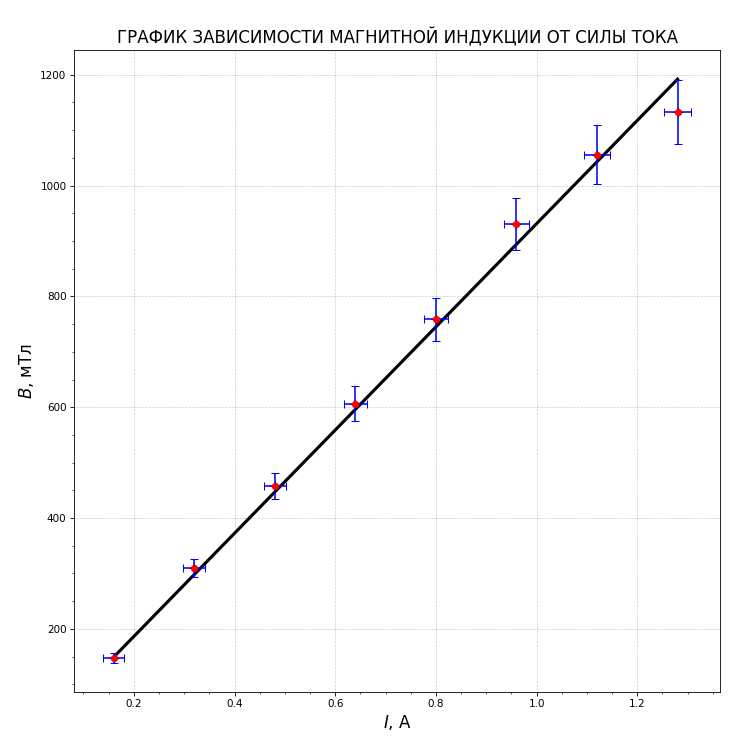
\includegraphics[width = 1.\textwidth]{B(I).png}
\end{figure}
\newpage

\begin{figure}[H]\label{fig: U(B)) Cu}
    \centering
    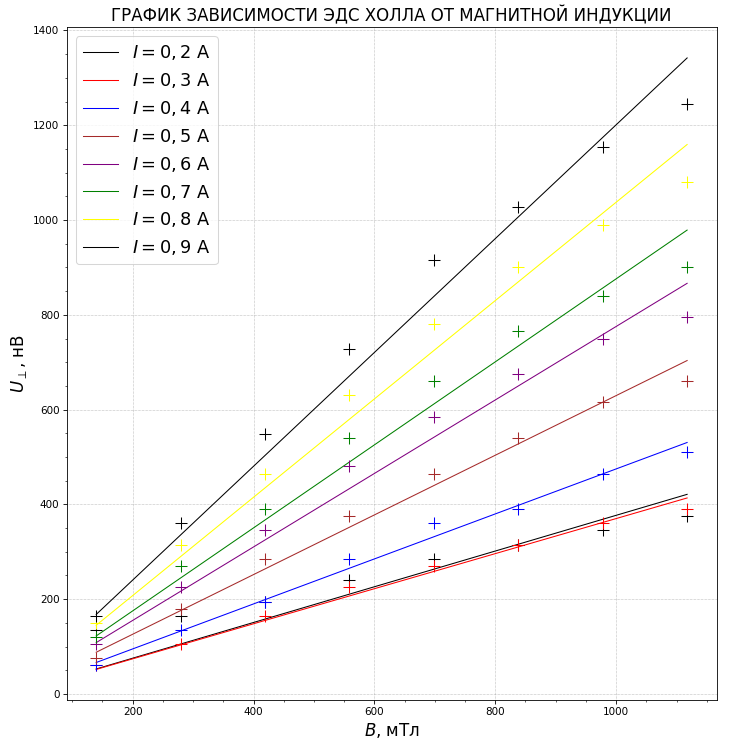
\includegraphics[width = 1.\textwidth]{U(B)_Cu.png}
\end{figure}
\newpage
\begin{figure}[H]\label{fig: k(I) Cu}
    \centering
    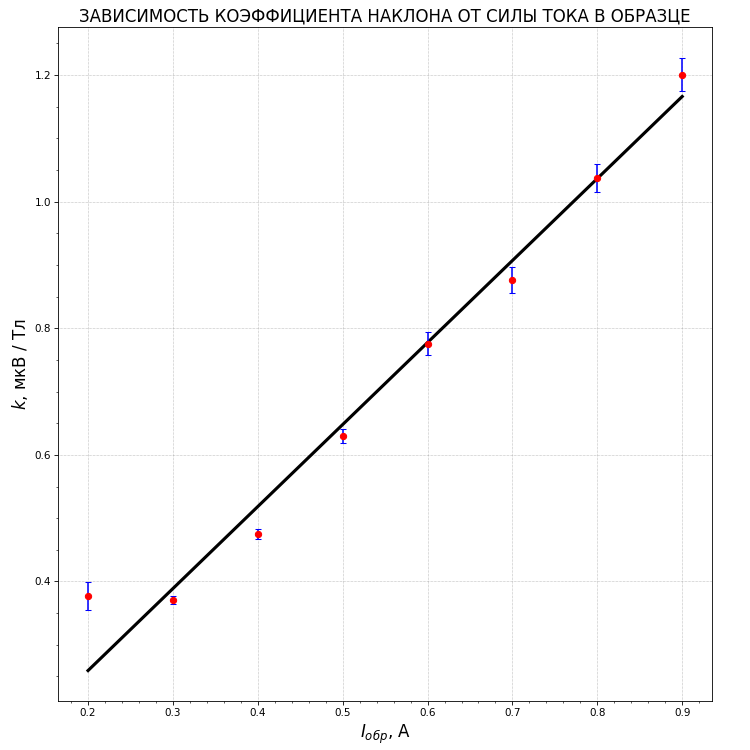
\includegraphics[width = 1.\textwidth]{k(I)_Cu.png}
\end{figure}
\newpage

\begin{figure}[H]\label{fig: U(B)) Zn}
    \centering
    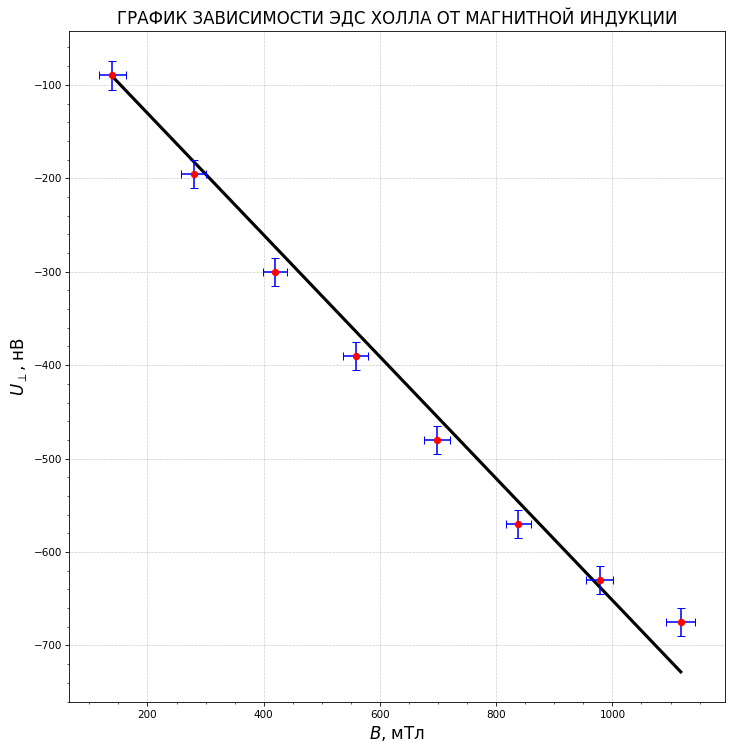
\includegraphics[width = 1.\textwidth]{U(B)_Zn.png}
\end{figure}
\newpage



\end{document}
